\documentclass[10pt]{beamer}
\usetheme[outer/progressbar=foot]{metropolis}
\usepackage{booktabs}
%\usepackage[scale=2]{ccicons}
\usepackage{pgfplots}
\usepackage{cancel}
\usepackage[ngerman]{babel}
\usepackage[utf8]{inputenc}
\usepackage{blindtext}
\usepackage{amsmath}
\usepackage[italicdiff]{physics}
\usepackage[italic]{hepnames}
\usepackage{graphicx}
\usepackage{float}
\usepackage{color}
\usepackage{mathtools}
\usepackage{physics}
\usepackage[absolute,overlay]{textpos}
\usepackage[texcoord,grid,gridcolor=red!10,subgridcolor=green!10,gridunit=pt]{eso-pic}

\usepackage{tikz}
\usetikzlibrary{trees}
\usetikzlibrary{decorations.pathmorphing}
\usetikzlibrary{decorations.markings}

\usepgfplotslibrary{dateplot}


%Frontpage
\title{Boundary Errors In Calorimetry}
\date{\today}
\author{Peter Schleper, \textbf{Simon Schnake}, Hartmut Stadie}
\institute{Universität Hamburg}

%Document
\begin{document}
\maketitle
\tikzstyle{every picture}+=[remember picture]

\begin{frame}{Deep Learning}
  \begin{textblock*}{150pt}(200pt,35pt)
    \begin{figure}[htp]
      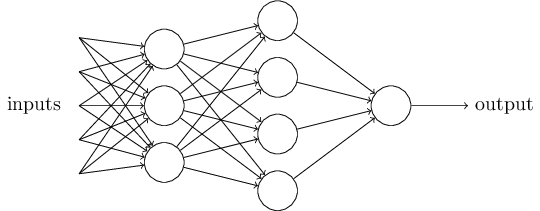
\includegraphics[width=\textwidth]{tikz1.png}
    \end{figure}
  \end{textblock*}
  \begin{textblock*}{150pt}(207pt,150pt)
    \Huge{$\}$}
  \end{textblock*}
  \begin{textblock*}{150pt}(225pt,158pt)
    \emph{Backpropagation}
  \end{textblock*}
  \begin{itemize}
  \item Pass input $X$ to the network
  \item Calculate output $\hat{Y}$ and difference\\ to true value $Y$ (loss function)
  \item Calculate gradient of the loss
  \item Use gradient to update weights $W, b$
  \end{itemize}
  \begin{textblock*}{150pt}(20pt,200pt)
  \begin{align*}
    &a^{[0]} \coloneqq X \\
    &a^{[l]} \coloneqq \sigma^{[l]}(W^{[l]} a^{[l-1]}+ b^{[l]})\\
    &\hat{Y}(X) \coloneqq a^{[L]}
  \end{align*}
\end{textblock*}

  \begin{textblock*}{170pt}(160pt,210pt)
  \begin{align*}
    &\text{\emph{Example Loss}:}\\
    &\mathcal{L}(\hat{Y}, Y) = (\hat{Y} - Y)^2
  \end{align*}
\end{textblock*}
\end{frame}

\begin{frame}{Electromagnetic Calorimeter}
  \begin{columns}
    \column{0.5\textwidth}
    \begin{itemize}
    \item shower building
      \begin{itemize}
      \item bremsstrahlung
      \item pair production
      \end{itemize}
    \item measure the energy of the particle shower (destructive)
    \item sampling or homogenous
    \item resolution of a calorimeter
      $\frac{\sigma}{E} = \frac{a}{\sqrt{E}} \otimes b \otimes \frac{c}{E} $
    \end{itemize}
    \column{0.5\textwidth}
    \begin{figure}[htp]
      \tikzset{
        photon/.style={decorate, decoration={snake}, draw=red},
        electron/.style={draw=black}
      }

      \begin{tikzpicture}[
        thick,
        % Set the overall layout of the tree
        level/.style={level distance=1.5cm},
        level 2/.style={sibling distance=2.6cm},
        level 3/.style={sibling distance=3.2cm}
        ]

        \filldraw[fill=brown!20!white, draw=black] (0.5, 1.75) rectangle (4.5,-3.5);
        \filldraw[fill=brown!30!white, draw=brown!30!white] (1.0, 1.70) rectangle (1.5, -3.45);
        \filldraw[fill=brown!30!white, draw=brown!30!white] (2.0, 1.70) rectangle (2.5, -3.45);
        \filldraw[fill=brown!30!white, draw=brown!30!white] (3.0, 1.70) rectangle (3.5, -3.45);
        \filldraw[fill=brown!30!white, draw=brown!30!white] (4.0, 1.70) rectangle (4.45, -3.45);
        
        \draw[electron] (0,0) -- (1,0);
        \draw (-0.15, 0) node {$e$};
        \draw[photon] (1,0) -- (1.7, -1.25);
        \draw[electron] (1,0) -- (2, 0.55);
        \draw[electron] (1.7, -1.25) -- (2.5, -1);
        \draw[electron] (1.7, -1.25) -- (2.5, -2.05);
        \draw[electron] (2, 0.55) -- (2.7, 0);
        \draw[photon] (2, 0.55) -- (3, 0.75);
        \draw[photon] (2.5, -2.05) -- (3.1, -2.);
        
        \draw[electron] (3, 0.75) -- (3.7, 1.25);
        \draw (3.85, 1.25) node {$e$};
        \draw[electron] (3, 0.75) -- (3.7, 0.45);
        \draw (3.85, 0.45) node {$e$};
        \draw[photon] (2.7, 0) -- (3.7, 0.1);
        \draw (3.85, 0.1) node {$\gamma$};
        \draw[electron] (2.7, 0) -- (3.7, -0.5);
        \draw (3.85, -0.5) node {$e$};
        \draw[electron] (2.5, -1) -- (3.7, -0.8);
        \draw (3.85, -0.8) node {$e$};
        \draw[photon] (2.5, -1) -- (3.7, -1.2);
        \draw (3.85, -1.2) node {$\gamma$};
        \draw[electron] (3.1, -2.) -- (3.7, -1.5);
        \draw (3.85, -1.5) node {$e$};
        \draw[photon] (3.3, -2.15) -- (3.7, -2);
        \draw (3.85, -2) node {$\gamma$};

        \draw[electron] (3.1, -2.) -- (3.7, -2.5);
        \draw (3.85, -2.5) node {$e$};
        \draw[electron] (2.5, -2.05) -- (3.7, -3.);
        \draw (3.85, -3.) node {$e$};

      \end{tikzpicture}

    \end{figure}

  \end{columns}
\end{frame}

\begin{frame}{Simulation Setup}
  \begin{textblock*}{220pt}(150pt, 40pt)
    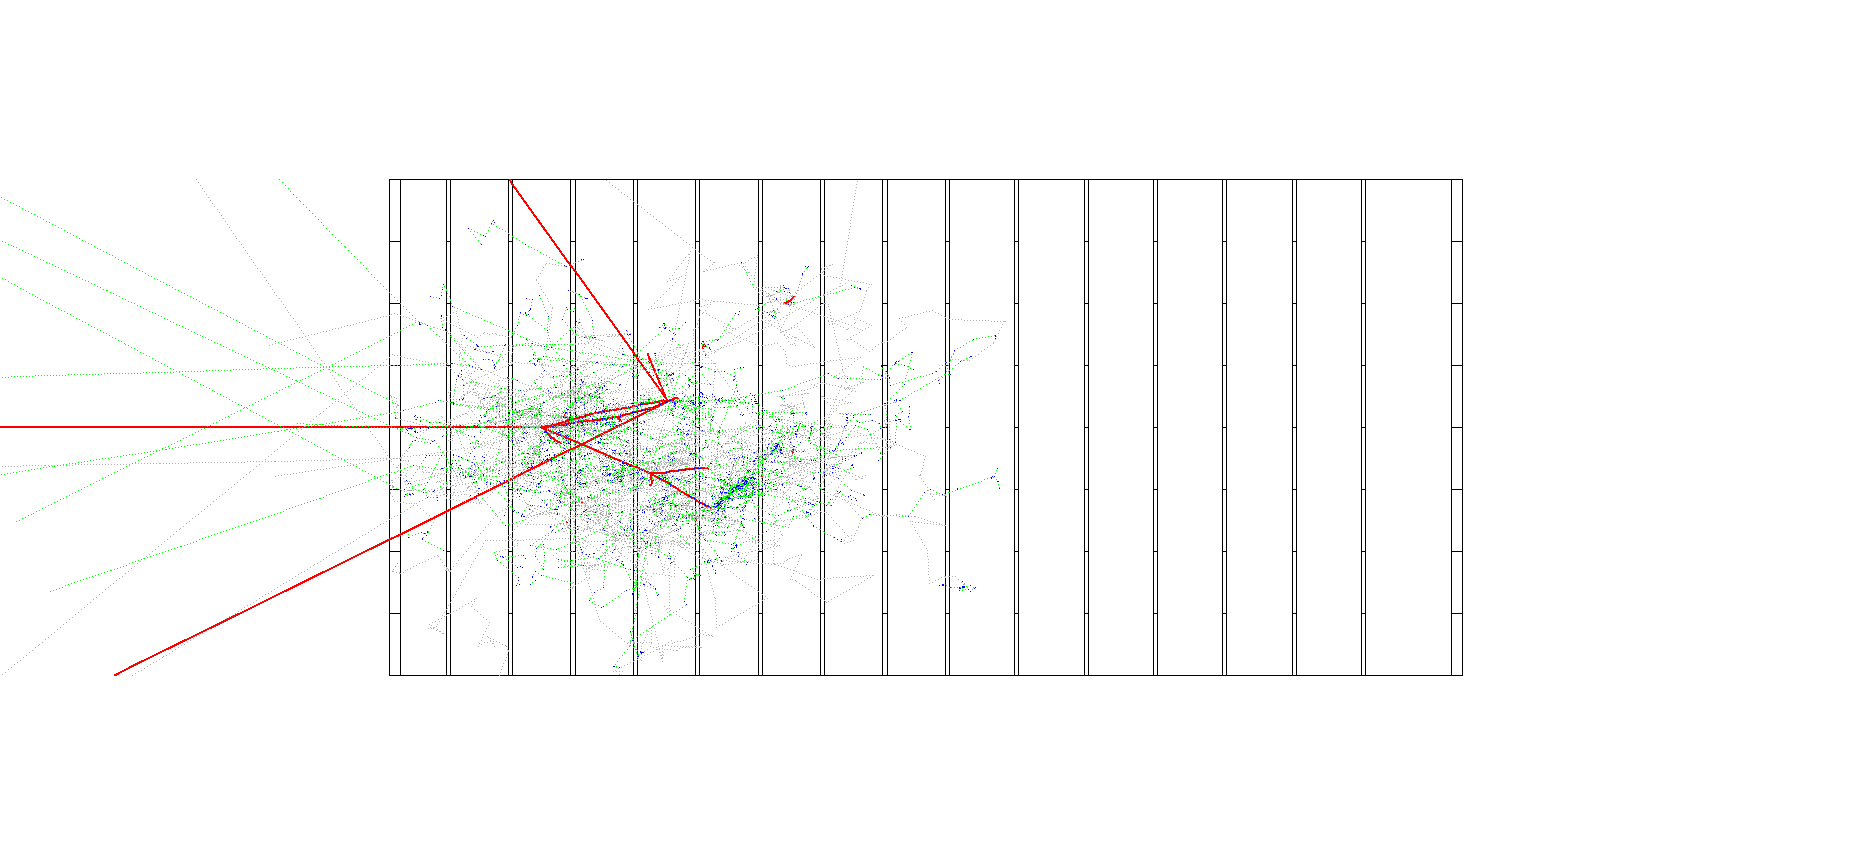
\includegraphics[width=\textwidth]{side.png}
  \end{textblock*}

  \begin{textblock*}{150pt}(2pt,100pt)
    \begin{itemize}
    \item Simulation with Geant4\small{}
    \item $e^-$ from 0. to 10 GeV
    \item 300,000 events
    \item 8x8x17 (1088) scint cells
    \item measure charged tracks in each scintillator cell
    \end{itemize}
  \end{textblock*}
  \begin{textblock*}{10pt}(170pt,150pt)
    \begin{tabular}{l|l|l}
      layer  & scint    & absorber \\ \hline
      layer 0      & 9mm     & 40 mm steel\\
      layer 1 - 8  & 3.7mm   & 50.5 mm brass \\
      layer 9 - 14 & 3.7mm   & 56.5 mm brass \\
      layer 15     & 3.7 mm  & 75 mm steel\\
      layer 16     & 9mm     &                      
    \end{tabular}
  \end{textblock*}
\end{frame}

\begin{frame}{Resulting Data}
  \begin{columns}
    \column{0.5\textwidth}
    \begin{figure}[htp]
      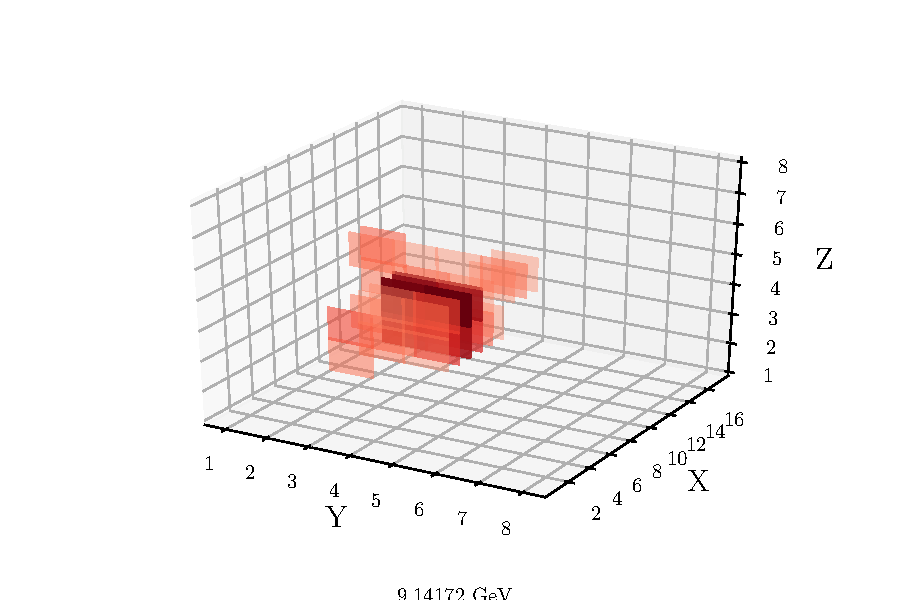
\includegraphics[width=1.1\textwidth]{../data_display.pdf}
    \end{figure}
    \column{0.5\textwidth}
    \begin{figure}[htp]
      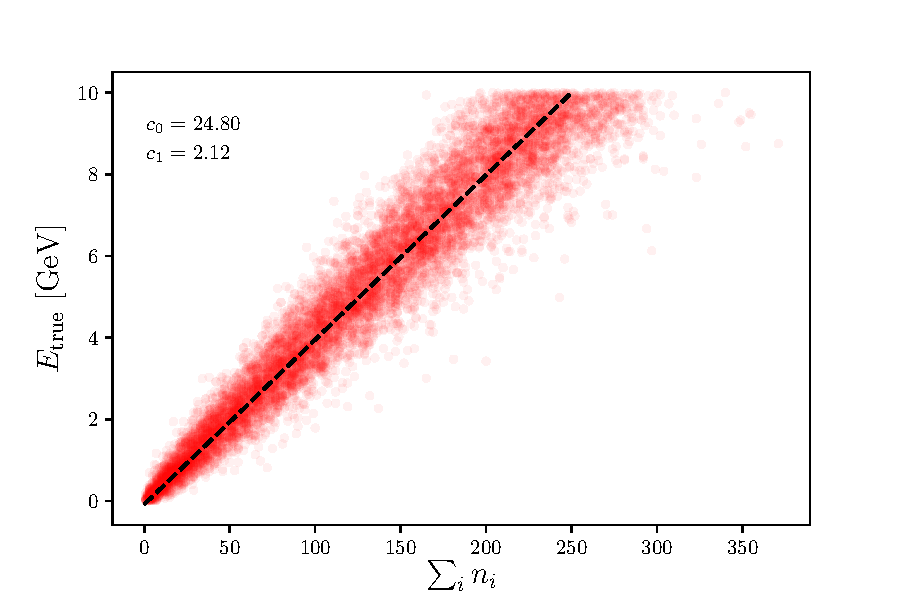
\includegraphics[width=\textwidth]{../e-vs-sum_n_fit.pdf}
    \end{figure}
  \end{columns}
\end{frame}

\begin{frame}{Neural Net}
  \begin{tabular}{l|l|l}
    Layer & Type                                & Activation \\ \hline
    1     & Conv3D(32, (2,2,2), strides = (1, 1, 1)) & ReLu       \\
    2     & Flatten()                           &            \\
    3-5   & Dense(128)                          & ReLu       \\
    6     & Dense(10)                           & ReLu       \\
    7     & Dense(1)                            & Linear    
  \end{tabular}
  \begin{itemize}
  \item Loss = Mean Squared Error
  \item Optimizer = RMSprop
  \item Data Augmentation with symmetry transformation (flipping, rotating and shifting)
  \end{itemize}
\end{frame}

\begin{frame}{Output Of The Neural Net}
  \begin{columns}
    \column{0.5\textwidth}
    \begin{figure}[htp]
      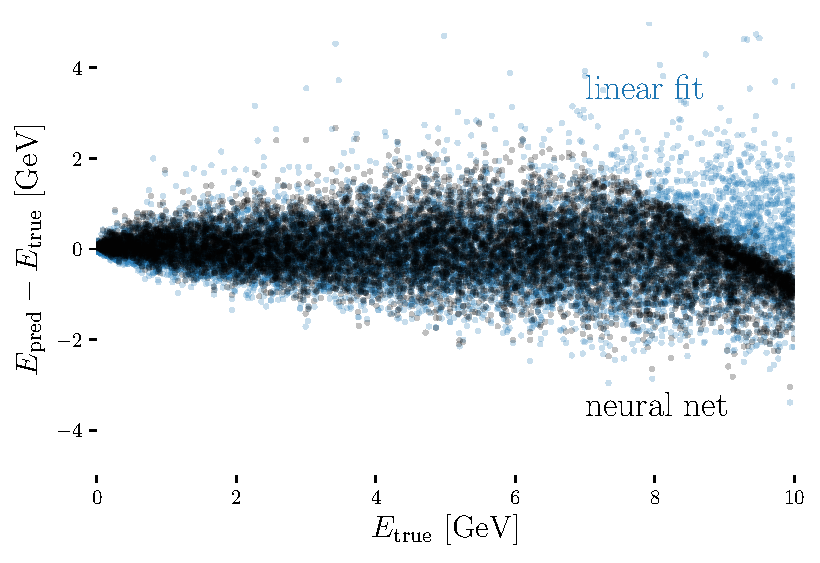
\includegraphics[width=1.1\textwidth]{../data_augment.pdf}
    \end{figure}
    \column{0.5\textwidth}
    \begin{figure}[htp]
      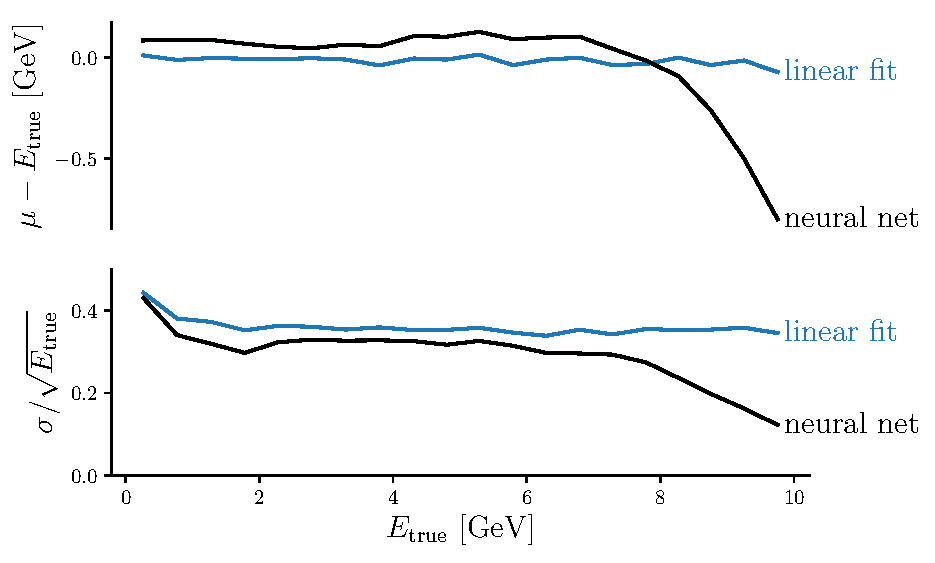
\includegraphics[width=1.1\textwidth]{../data_augment_res.pdf}
    \end{figure}
  \end{columns}
\end{frame}

\begin{frame}{Maximum Likelihood To Mean Squared Error}
Assumption: true values are gaussian distributed with const std $\sigma$
  \begin{align*}
    \text{max log likelihood} &= \text{max} \ln( \prod \frac{1}{\sqrt{2\pi \sigma^2}} e^{-\frac{(y_{\text{true}}-y_{\text{pred}})^2}{2 \sigma^2}}) \\
                              & =\text{max} \sum -\frac{(y_{\text{true}}-y_{\text{pred}})^2}{2 \sigma^2} - \ln(\sqrt{2\pi \sigma^2}) \\
                              & =-\text{max} \sum\frac{(y_{\text{true}}-y_{\text{pred}})^2}{\cancel{2 \sigma^2}} + \cancel{\ln(\sqrt{2\pi \sigma^2})} \\
                              & = \text{min} \sum (y_{\text{true}}-y_{\text{pred}})^2
  \end{align*}
\end{frame}

\begin{frame}{Maximum Likelihood Loss}
  \begin{textblock*}{150pt}(30pt,35pt)
      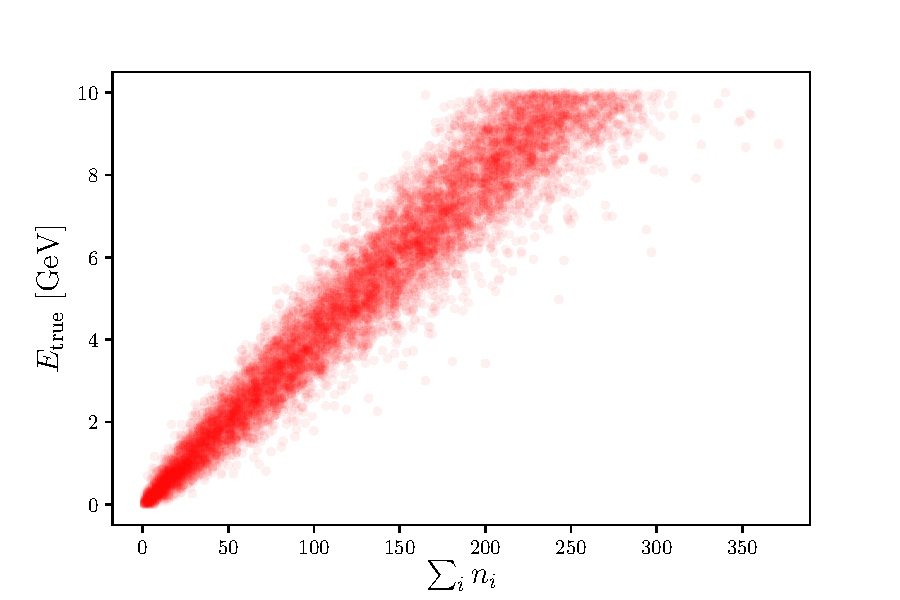
\includegraphics[width=\textwidth]{../e-vs-sum_n.pdf}
  \end{textblock*}
  \begin{textblock*}{150pt}(175pt,35pt)
    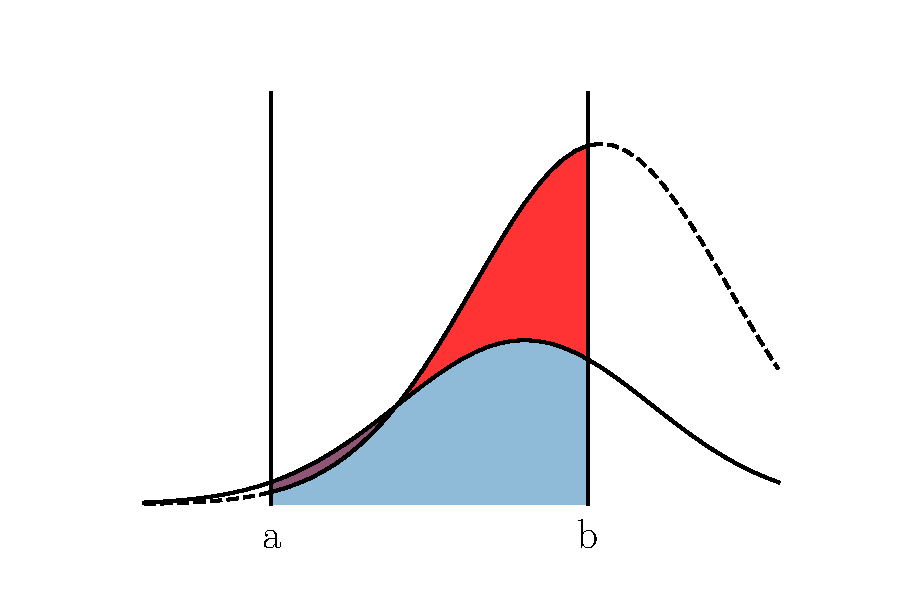
\includegraphics[width=\textwidth]{./gaussian_shift.pdf}
  \end{textblock*}

  \begin{textblock*}{150pt}(5pt,140pt)
    \begin{align*}
      \Rightarrow \text{max log likelihood} &= -\text{min} \sum \ln(\frac{\text{Norm}(y_{\text{true}} | y_{\text{pred}}, \sigma)}{\int^b_a \text{Norm}(y_{\text{true}} | y_{\text{pred}}, \sigma)})\\
                                            &=\ \text{min} \sum \frac{(y_{\text{true}}-y_{\text{pred}})^2}{2 \sigma^2}\\
   &\qquad \qquad +\ln(\frac{1}{2} \left(\text{erf}(\frac{y_{\text{pred}}-a}{\sqrt{2}\sigma}) - \text{erf}(\frac{y_{\text{pred}}-b}{\sqrt{2}\sigma})\right))
    \end{align*}
  \end{textblock*}
\end{frame}

\begin{frame}{Maximum Likelihood Loss}
  \begin{textblock*}{150pt}(150pt,55pt)
    $\sigma = 0.31 \sqrt{y_{\text{true}}}$
  \end{textblock*}
  \begin{columns}
    \column{0.5\textwidth}
    \begin{figure}[htp]
      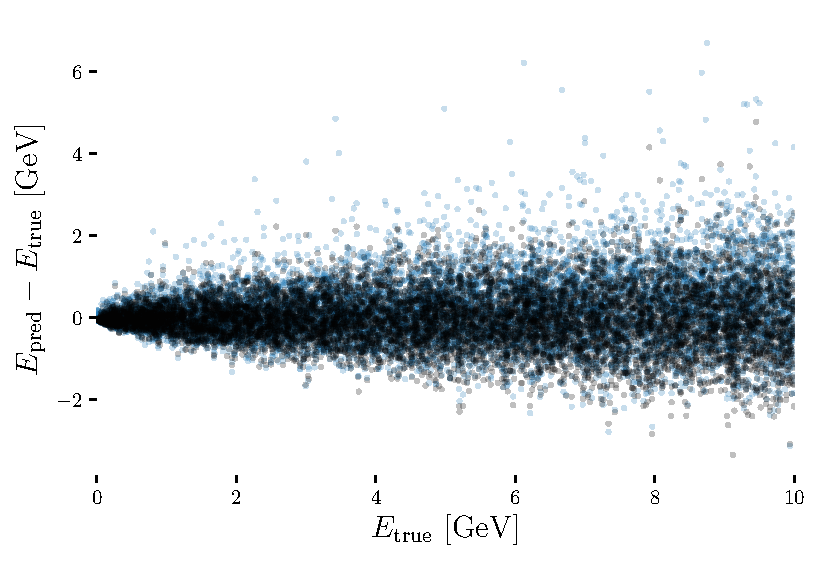
\includegraphics[width=1.1\textwidth]{../likelihood.pdf}
    \end{figure}
    \column{0.5\textwidth}
    \begin{figure}[htp]
      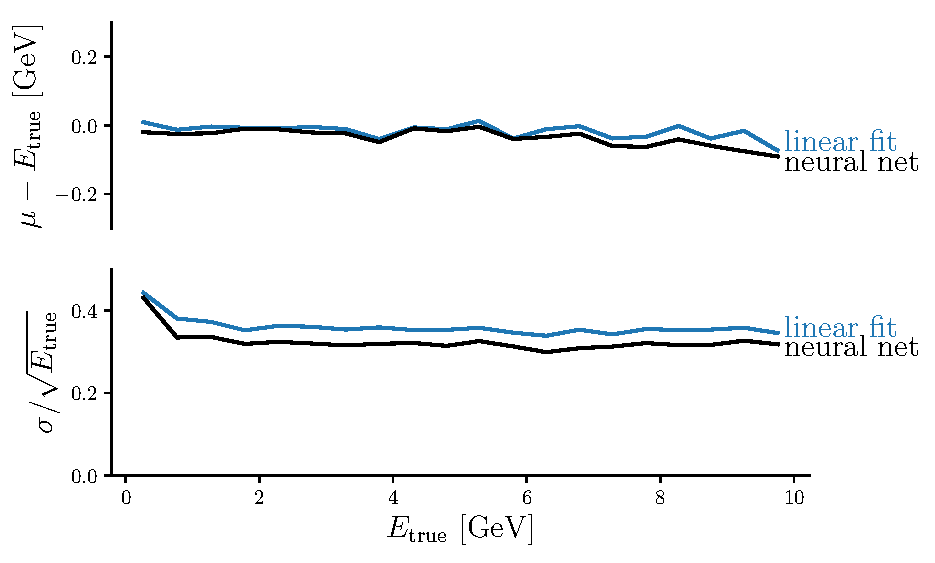
\includegraphics[width=1.1\textwidth]{../likelihood_res.pdf}
    \end{figure}
  \end{columns}
\end{frame}

\begin{frame}{Summary}
  \begin{itemize}
  \item Brief discussion of deep learning and calorimetry 
  \item Simulation of a calorimeter
  \item Presentation of a typical border problem
  \item Solution by a  customized loss function
  \end{itemize}
\end{frame}

\end{document}
